\documentclass[12pt]{beamer}
\usetheme{moloch}

\usepackage{amsmath,amscd}
\usepackage{fontspec}
\usepackage{unicode-math}
\usepackage[dvipsnames]{xcolor}
\usepackage{tikz}
\usepackage{pgfplots}
\pgfplotsset{compat=1.18}
\usetikzlibrary{positioning}
\usepackage{booktabs}
\usepackage{array}
\usetikzlibrary{arrows.meta,fit,backgrounds}

\setbeamercolor{background canvas}{bg=black}
\setbeamercolor{normal text}{fg=white}

\setmonofont{DejaVu Sans Mono}

% Set the title bar to black background with white text
\setbeamercolor{frametitle}{bg=black, fg=white}

% Ensure other structural elements (bullets, etc.) are visible
\setbeamercolor{structure}{fg=white}

\iffalse
%\usepackage{ebgaramond}
\setmainfont{texgyrepagella}[
  Extension = .otf,
  UprightFont = *-regular,
  BoldFont = *-bold,
  ItalicFont = *-italic,
  BoldItalicFont = *-bolditalic,
  Color=charcoal,
]
\setmathfont{texgyrepagella-math.otf}
\fi

\iftrue
\setmainfont{Libertinus Serif}
\setsansfont{Libertinus Sans}
\setmonofont{DejaVu Sans Mono}
\setmathfont{STIXTwoMath-Regular.otf}
\fi

% Define colors for syntax highlighting
\definecolor{codegreen}{rgb}{0,0.6,0}
\definecolor{codegray}{rgb}{0.5,0.5,0.5}
\definecolor{codecoffee}{rgb}{0.75,0.6,0.3}
\definecolor{question}{rgb}{1.0,0.75,0.1}
\definecolor{lightblue}{rgb}{0.55,0.75,0.9}
\definecolor{yellow}{rgb}{1.0, 1.0, 0.0}
\definecolor{codecomment}{rgb}{0.97, 0.74, 0.4}
\definecolor{codepy}{rgb}{0.9, 0.85, 0.85} %{#F8BC65}
\definecolor{funcColor}{rgb}{0.47, 0.6, 0.8}
\definecolor{midgray}{rgb}{0.4, 0.4, 0.3}
\definecolor{indexwhite}{rgb}{0.9, 0.9, 0.9}

\newcommand{\FrameTitle}[2]{\frametitle{#1 \hfill \small\textnormal{\textcolor{midgray}{#2}}}}
\newcommand{\snl}{\vspace*{4pt}\\}
\newcommand{\nl}{\vspace*{1em}\\}
\newcommand{\vsp}{\vspace*{1em}}
\newcommand{\SixPtVspace}{\vspace*{6pt}}

\newcommand{\Quiz}[1]{{\large\textbf{\color{question}{#1}}}}
\newcommand{\QuizQuestion}[1]{{\Large\textbf{\color{question}{#1}}}}

\newcommand{\Matrix}[1]{\textbf{#1}}
\newcommand{\Vector}[1]{\textbf{#1}}
\newcommand{\MMat}[1]{\mathbf{#1}}
\newcommand{\MVec}[1]{\mathbf{#1}}
\newcommand{\Norm}[1]{\lVert {\mathbf{#1}} \rVert}
\newcommand{\NormBeta}[1]{\lVert \beta \mathbf{#1} \rVert}
\newcommand{\NormConst}[1]{\lVert #1 \rVert}
\newcommand{\Trans}{\text{\raisebox{0.5ex}{\scalebox{0.75}{T}}}}
\newcommand{\abs}[1]{\lvert {#1} \rvert}
\newcommand{\Avg}[1]{\mathbf{avg}(\mathbf{#1})}
\newcommand{\Std}[1]{\mathbf{std}(\mathbf{#1})}


\begin{document}
\title{\center{Applied Linear Algebra\vspace*{4pt}\\Unit 3\\}}
\author{\center{Devi Prasad M \\ Manipal School of Information Sciences \\ Manipal \\}}
\date{\center{October 2026}}
\maketitle

\begin{frame}\FrameTitle{Topics and Time Allocation}{Unit 3}
    %\vspace*{-1em}
    \begin{itemize}
        \item Derivatives in one dimension \hfill (0.5 h)%
        \item Gradients in multiple dimensions \hfill (1 h)%
        \item Chain rule in multiple dimensions \hfill (1 h)%
        \item Gradients of matrix expressions \hfill (2 h)%
        \item Optimization using gradient descent \hfill(3.5 h)%
        \begin{itemize}
            \item single-sample updates
            \item Logistic regression (No hidden layer)
            \item Softmax regression (No hidden layer)
        \end{itemize}
        \item Backpropagation \hfill (3 h)%
        \begin{itemize}
            \item Computational graphs
            \item Multi-layer perceptrons (Hidden Layers)
        \end{itemize}
    \end{itemize}
\end{frame}


\begin{frame}\FrameTitle{Training a Network Using PyTorch}{Unit 3}
    \centerline{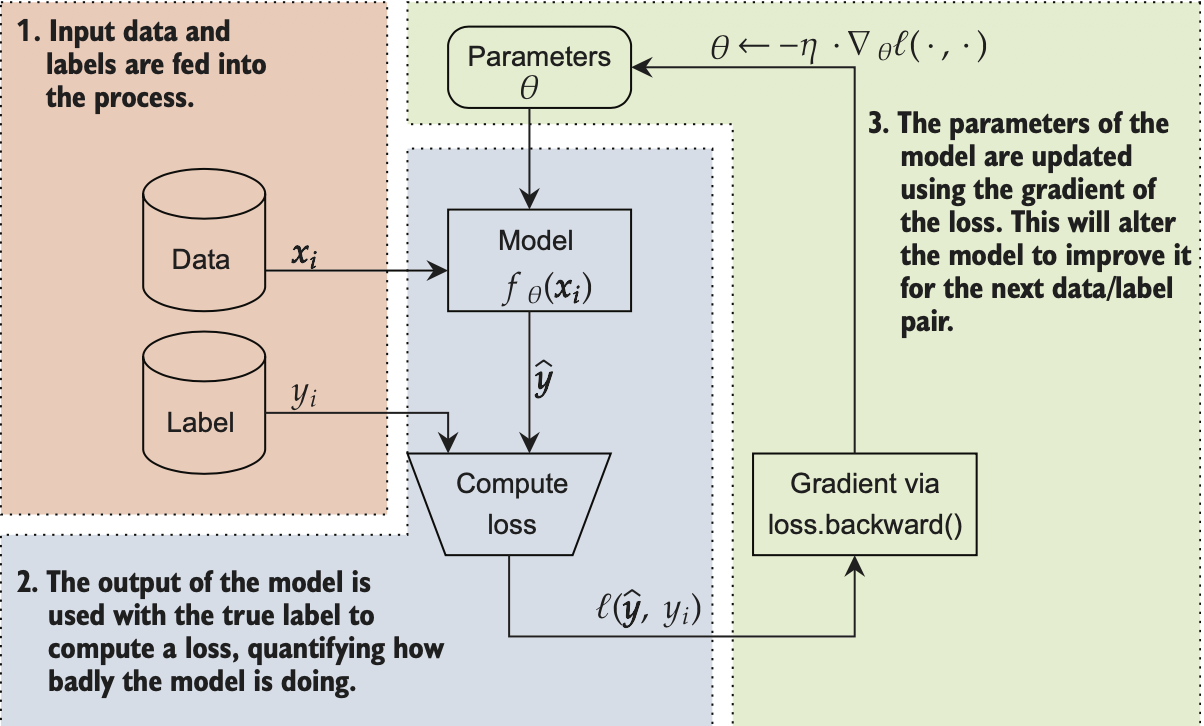
\includegraphics[width=0.97\linewidth]{figures/dl-train-01.png}}
\end{frame}


\begin{frame}\FrameTitle{Training a Network Using PyTorch}{Unit 3}
    \centerline{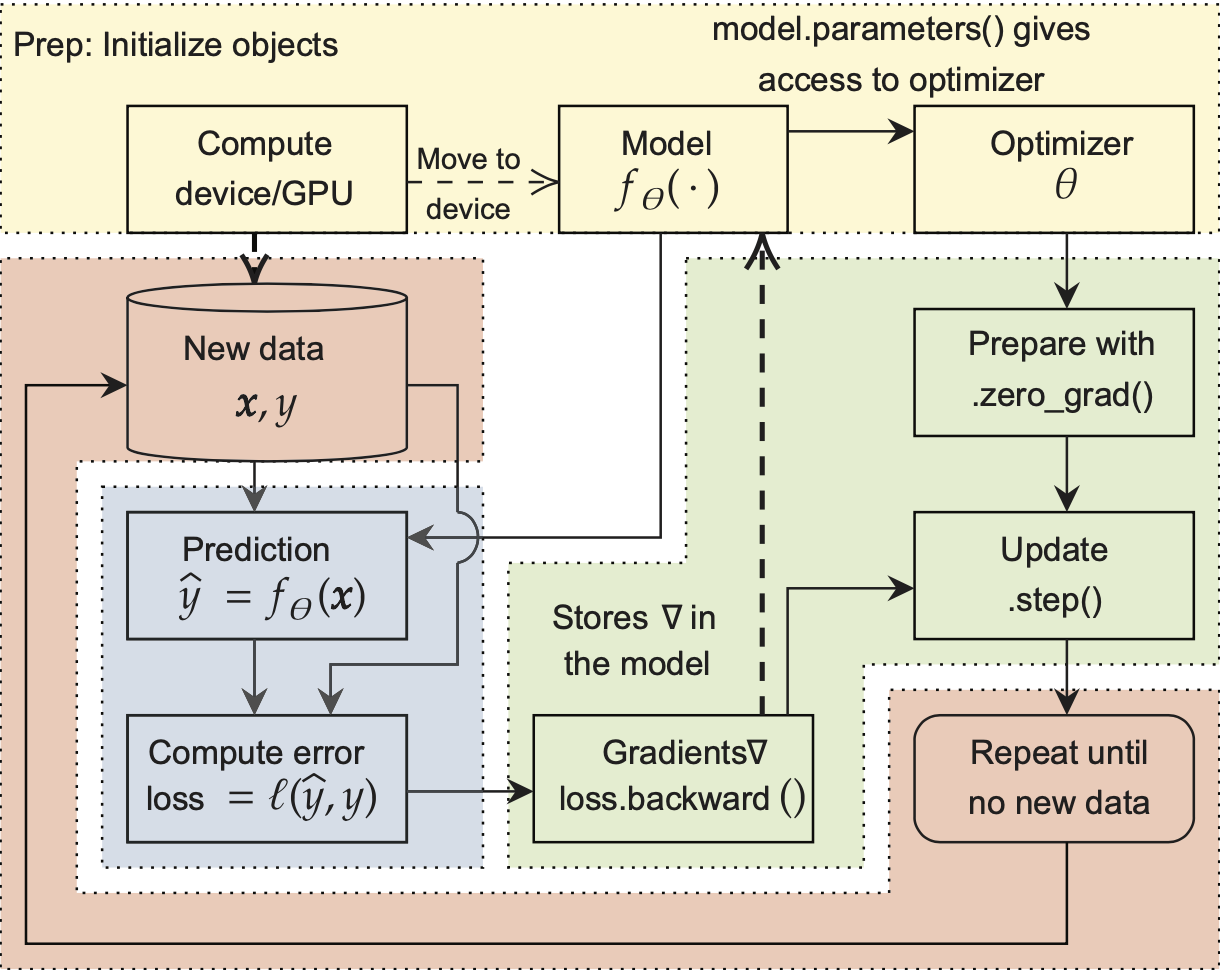
\includegraphics[width=0.9\linewidth]{figures/dl-train-02.png}}
\end{frame}

\begin{frame}\FrameTitle{Where gradients are computed and used}{Unit 3}
    \centering
    \resizebox{0.74\linewidth}{!} {%
    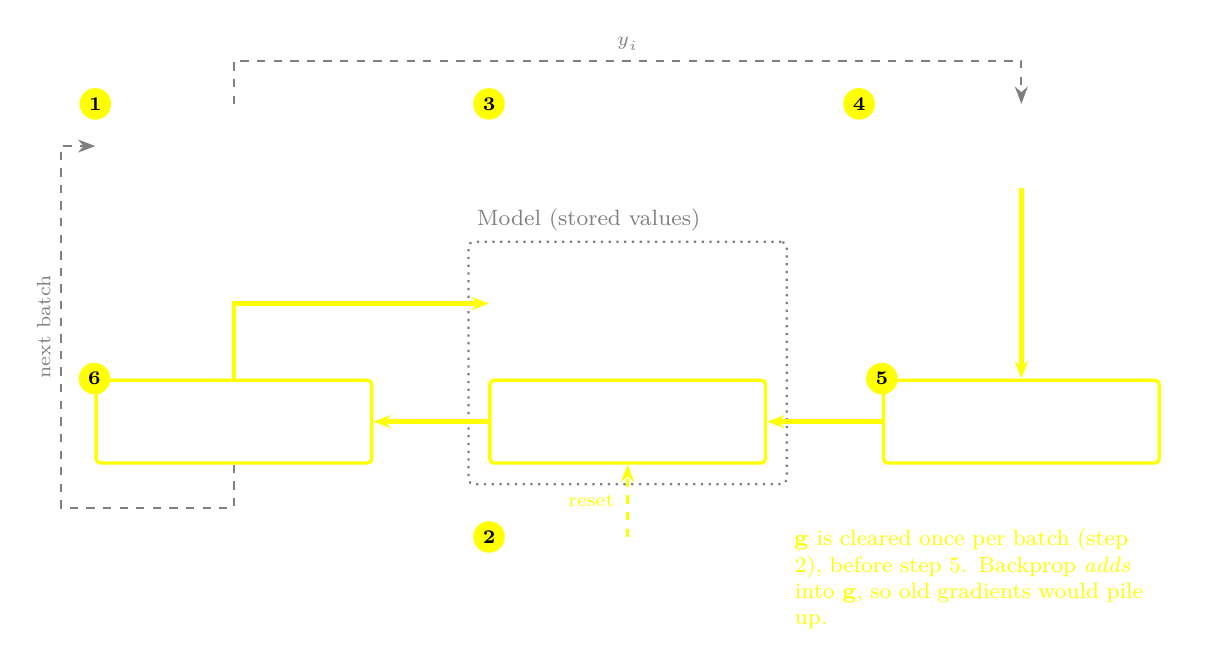
\begin{tikzpicture}[
        font=\small, >={Stealth[length=2.2mm]},
        box/.style={draw=white, line width=0.6pt, rounded corners=1.5pt, minimum width=3.5cm,
                    minimum height=1.05cm, align=center, text=white},
        gbox/.style={box, draw=yellow, line width=1.2pt},
        flow/.style={->, white, line width=0.7pt},
        gflow/.style={->, yellow, line width=1.6pt},
        dflow/.style={->, gray, dashed, line width=0.7pt},
        num/.style={circle, fill=yellow, text=black, inner sep=0pt, minimum size=4mm,
                    font=\scriptsize\bfseries},
        note/.style={font=\footnotesize, text=yellow, align=left}]

        % ---- nodes ----
        \node[box]  (data) at (0,0)    {Data batch of $B$\\[-1pt]pairs $(\symbf{x}_i,y_i)$};
        \node[box]  (fwd)  at (5,0)    {Forward pass\\[-1pt]$\hat y_i=f_{\symbf{\theta}}(\symbf{x}_i)$};
        \node[box, minimum width=4.1cm]  (loss) at (10,0)   {Loss (batch average)\\[-1pt]$L=\tfrac1B\sum_{i=1}^{B}\ell(\hat y_i,y_i)$};
        \node[box]  (th)   at (5,-2.0) {Parameters $\symbf{\theta}$};
        \node[gbox] (g)    at (5,-3.5) {Gradient buffer $\symbf{g}$};
        \node[gbox] (bp)   at (10,-3.5){Backpropagation\\[-1pt]$\symbf{g}\mathrel{+}=\nabla_{\symbf{\theta}}L$};
        \node[gbox] (upd)  at (0,-3.5) {Optimizer update\\[-1pt]$\symbf{\theta}\leftarrow\symbf{\theta}-\eta\,\symbf{g}$};
        \node[box]  (clr)  at (5,-5.5) {Clear the buffer\\[-1pt]$\symbf{g}\leftarrow\symbf{0}$};

        % model container
        \begin{scope}[on background layer]
            \node[draw=gray, dotted, line width=0.8pt, rounded corners=2pt, inner sep=2.5mm,
                fit=(th)(g)] (model) {};
        \end{scope}
        \node[font=\footnotesize, text=gray, anchor=south west] at (model.north west) {Model (stored values)};

        % ---- arrows ----
        \draw[flow]  (data) -- node[above,font=\scriptsize]{$\symbf{x}_i$} (fwd);
        \draw[flow]  (fwd)  -- node[above,font=\scriptsize]{$\hat y_i$} (loss);
        \draw[dflow] (data.north) -- ++(0,0.55) -| node[above,pos=0.25,font=\scriptsize]{$y_i$} (loss.north);
        \draw[flow]  (th.north) -- (fwd.south);            % forward reads theta
        \draw[gflow] (loss.south) -- (bp.north);            % loss starts the backward pass
        \draw[gflow] (bp.west) -- (g.east);                 % backprop writes g
        \draw[gflow] (g.west) -- (upd.east);                % update reads g
        \draw[gflow] (upd.north) |- (th.west);              % update writes theta
        \draw[->, yellow, dashed, line width=1.2pt] (clr.north) -- node[left,font=\scriptsize,text=yellow,inner sep=1.5mm]{reset} (g.south);   % clear g
        \draw[dflow] (upd.south) -- ++(0,-0.55) -- ++(-2.2,0) |- (data.west)
                node[pos=0.25,above,sloped,font=\scriptsize,text=gray]{next batch};

        % ---- step badges (execution order) ----
        \node[num] at (data.north west) {1};
        \node[num] at (clr.north west)  {2};
        \node[num] at (fwd.north west)  {3};
        \node[num] at (loss.north west) {4};
        \node[num] at (bp.north west)   {5};
        \node[num] at (upd.north west)  {6};

        % ---- notes ----
        \node[note, anchor=west, text width=4.6cm] at (7.0,-5.5) {\hyphenpenalty=10000 \exhyphenpenalty=10000 $\symbf{g}$ is cleared once per batch (step 2), before step 5. Backprop \emph{adds} into $\symbf{g}$, so old gradients would pile up.\par};
    \end{tikzpicture}}
    \vfill
    {\color{yellow}\rule{\linewidth}{0.5pt}}\par\vspace{1mm}
    {\raggedright\small\textcolor{yellow}{\textbf{In an LLM:}}
        a batch is $B$ token sequences; steps 3--5 run once per batch,
        not once per sample, and give one gradient entry per parameter,
        billions in all.\par}
\end{frame}

% ============================================================ GPT-2
\begin{frame}\FrameTitle{GPT-2: one batch in numbers}{Unit 3}
    \vspace*{-3mm}
    \begin{columns}[T]
        \begin{column}{0.45\linewidth}
        \centering
            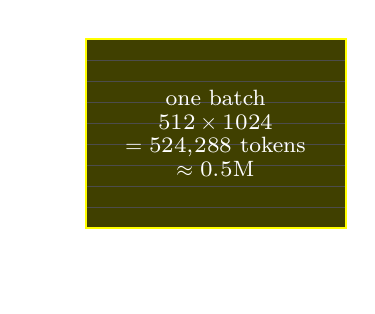
\begin{tikzpicture}[font=\footnotesize]
                \def\w{3.3}\def\h{2.4}
                \fill[yellow!25!black] (0,0) rectangle (\w,\h);
                \foreach \i in {1,...,8} \draw[gray!60!black,line width=0.3pt] (0,\i*\h/9) -- (\w,\i*\h/9);
                \draw[yellow,line width=0.8pt] (0,0) rectangle (\w,\h);
                \draw[<->,white] (-0.25,0) -- node[left,rotate=90,anchor=south]{$B=512$ sequences} (-0.25,\h);
                \draw[<->,white] (0,-0.25) -- node[below]{$1{,}024$ tokens each} (\w,-0.25);
                \node[text=white,align=center] at (\w/2,\h/2) {one batch\\[-1pt]$512\times1024$\\[-1pt]$=524{,}288$ tokens\\[-1pt]$\approx0.5$M};
            \end{tikzpicture}
        \end{column}
        \begin{column}{0.53\linewidth}
            \footnotesize
            \begin{tabular}{@{}rrr@{}}
            \textcolor{yellow}{\textbf{Parameters}} & \textcolor{yellow}{\textbf{Layers}} & \textcolor{yellow}{\textbf{$d_{\text{model}}$}} \\
            117M & 12 & 768 \\ 345M & 24 & 1024 \\ 762M & 36 & 1280 \\ 1542M & 48 & 1600
            \end{tabular}
            \begin{itemize}\footnotesize\setlength{\itemsep}{1.2mm}
                \item ``a larger batchsize of 512 is used''; context raised from 512 to 1,024 tokens.
                \item Vocabulary $50{,}257$; WebText: about 8M documents, 40\,GB.
                \item Learning rate ``manually tuned'' for each model.
            \end{itemize}
        \end{column}
    \end{columns}
    {\par\vspace{1mm}\footnotesize\textcolor{gray}
        {Radford et al.\ (2019), Sec.\ 2.3 and Table 2.
            Total training tokens are not stated in the paper.}\par}
    \vfill
    {\color{yellow}\rule{\linewidth}{0.5pt}}\par\vspace{1mm}
    {\raggedright\small\textcolor{yellow}{\textbf{In an LLM:}}
        one forward pass, one backward pass and one update
        $\symbf{\theta}\leftarrow\symbf{\theta}-\eta\,\symbf{g}$
        per batch of about $0.5$M tokens.\par}
\end{frame}

% ============================================================ GPT-3
\begin{frame}\FrameTitle{GPT-3: the batch grows with the model}{Unit 3}
    \centering\footnotesize
    \begin{tabular}{@{}lrrrrr@{}}
        \textcolor{yellow}{\textbf{Parameters}} & \textcolor{yellow}{\textbf{Layers}} & \textcolor{yellow}{\textbf{$d_{\text{model}}$}} &
        \textcolor{yellow}{\textbf{Batch (tokens)}} & \textcolor{yellow}{\textbf{Peak LR}} & \textcolor{yellow}{\textbf{Updates $\approx$}}\\[0.5mm]
        125M & 12 & 768   & 0.5M & $6.0\times10^{-4}$ & 600{,}000\\
        350M & 24 & 1024  & 0.5M & $3.0\times10^{-4}$ & 600{,}000\\
        760M & 24 & 1536  & 0.5M & $2.5\times10^{-4}$ & 600{,}000\\
        1.3B & 24 & 2048  & 1M   & $2.0\times10^{-4}$ & 300{,}000\\
        2.7B & 32 & 2560  & 1M   & $1.6\times10^{-4}$ & 300{,}000\\
        6.7B & 32 & 4096  & 2M   & $1.2\times10^{-4}$ & 150{,}000\\
        13B  & 40 & 5140  & 2M   & $1.0\times10^{-4}$ & 150{,}000\\
        175B & 96 & 12288 & 3.2M & $0.6\times10^{-4}$ & 94{,}000
    \end{tabular}
    \par%\vspace{2mm}
    \begin{flushleft}\small
        Context $2{,}048$ tokens; $300$B training tokens for every model. Updates $\approx$ tokens\,/\,batch.\\
        Larger model $\Rightarrow$ larger batch, \emph{smaller} learning rate: the paper notes this trend.
    \end{flushleft}
    {\par\vspace{1mm}\footnotesize\textcolor{gray}{
            Brown et al.\ (2020), Table 2.1.
            The ``Updates'' column is derived.}\par}
    \vfill
    {\color{yellow}\rule{\linewidth}{0.5pt}}\par\vspace{1mm}
    {\raggedright\small\textcolor{yellow}{\textbf{In an LLM:}}
        at 175B, a batch of $3.2$M tokens is about $1{,}560$
        sequences, and training is only about $94{,}000$
        updates.\par}
\end{frame}

% ============================================================ Llama 2 and 3
\begin{frame}\FrameTitle{Llama 2 and Llama 3: Millions of Tokens per Update}{}
\vspace*{-3mm}
\begin{columns}[T]
\begin{column}{0.47\linewidth}
  \textcolor{yellow}{\textbf{Llama 2 (7B to 70B)}}
  \begin{itemize}\footnotesize\setlength{\itemsep}{1.2mm}
    \item Global batch $4$M tokens, context $4{,}096$, $2$T tokens in all: about $500{,}000$ updates.
    \item AdamW, cosine schedule, $2{,}000$ warmup steps, gradient clipping $1.0$.
    \item Peak LR $3\times10^{-4}$ (7B, 13B) and $1.5\times10^{-4}$ (34B, 70B).
  \end{itemize}
\end{column}
\begin{column}{0.50\linewidth}
  \textcolor{yellow}{\textbf{Llama 3 405B: the batch is ramped up}}
  \vspace{1mm}
  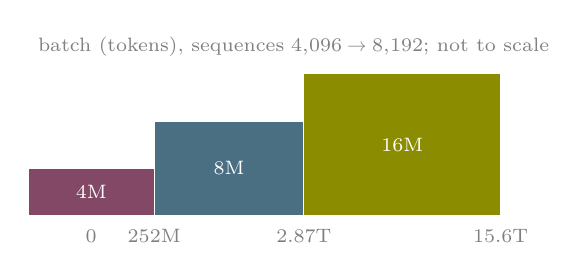
\begin{tikzpicture}[font=\scriptsize, x=1cm, y=1cm]
    \draw[fill=magenta!45!black,draw=white] (0,0) rectangle (1.6,0.6);
    \draw[fill=cyan!45!black,draw=white]    (1.6,0) rectangle (3.5,1.2);
    \draw[fill=yellow!55!black,draw=white]  (3.5,0) rectangle (6.0,1.8);
    \node[white] at (0.8,0.3) {4M};
    \node[white] at (2.55,0.6) {8M};
    \node[white] at (4.75,0.9) {16M};
    \node[gray,anchor=north,align=center] at (0.8,-0.05) {0};
    \node[gray,anchor=north,align=center] at (1.6,-0.05) {252M};
    \node[gray,anchor=north,align=center] at (3.5,-0.05) {2.87T};
    \node[gray,anchor=north,align=center] at (6.0,-0.05) {15.6T};
    \node[gray,anchor=south west] at (0,1.9) {batch (tokens), sequences $4{,}096\to8{,}192$; not to scale};
  \end{tikzpicture}
  \vspace*{-2mm}
  \begin{itemize}\footnotesize\setlength{\itemsep}{1.2mm}
    \item AdamW, peak LR $8\times10^{-5}$, $8{,}000$ warmup steps, cosine decay to $8\times10^{-7}$.
  \end{itemize}
\end{column}
\end{columns}
{\par\vspace{2mm}\footnotesize\textcolor{gray}
    {Touvron et al.\ (2023), Sec.\ 2.2; Llama Team (2024),
     Sec.\ 3.4.1. The Llama 3 paper says ``8M sequences
     of 8,192 tokens''; read here as $8$M tokens.}\par}
\vspace*{-3mm}
{\color{yellow}\rule{\linewidth}{0.5pt}}\par\vspace{1mm}
{\raggedright\small\textcolor{yellow}{\textbf{In an LLM:}}
    the batch size is not fixed: it is raised during training,
    alongside the learning-rate schedule.\par}
\end{frame}


% ============================================================ why B is a hyperparameter
\begin{frame}\FrameTitle{Why the batch size is a hyperparameter}{Unit 3}
\begin{columns}[T]
\begin{column}{0.40\linewidth}
  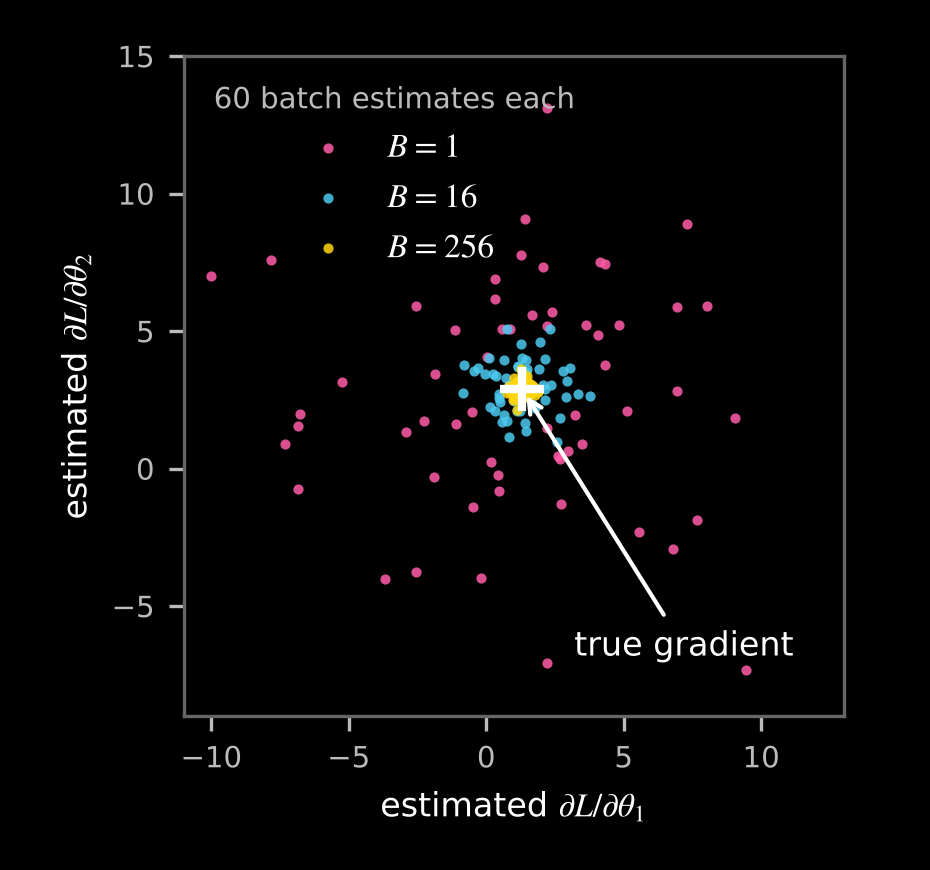
\includegraphics[width=\linewidth]{figures/s8_batchnoise.png}
\end{column}
\vspace*{-4mm}
\begin{column}{0.62\linewidth}
  \begin{itemize}\footnotesize\setlength{\itemsep}{1.4mm}
    \item \textbf{Gradient quality.} $\symbf{g}$ is an average over $B$ samples. The scatter shrinks roughly like $1/\sqrt{B}$ (synthetic example, same true gradient).
    \item \textbf{Learning rate.} The best $\eta$ depends on $B$; GPT-3 pairs larger batches with smaller learning rates.
    \item \textbf{Cost.} Memory and hardware grow with $B$.
    \item \textbf{Number of updates.} With a fixed token budget, updates $\approx$ tokens\,/\,$B$.
    \item \textbf{Does not fit?} Split the batch into micro-batches and keep $\symbf{g}$ (do not clear it) until the last one: gradient accumulation.
  \end{itemize}
\end{column}
\end{columns}
%\vfill
%{\color{yellow}\rule{\linewidth}{0.5pt}}\par\vspace{1mm}
%{\raggedright\small\textcolor{yellow}{\textbf{In an LLM:}} $B$ is chosen before training, like $\eta$, and often changed on a schedule.\par}

\end{frame}

\begin{frame}\FrameTitle{Learning is optimization in high dimensions}{Unit 3}
{\small A deep network has $N$ adjustable parameters $\symbf{\theta}$ (billions in an LLM).
A loss $L(\symbf{\theta})$ scores it on training data; training finds $\symbf{\theta}$ with
small $L$ by going downhill in $\symbb{R}^{N}$.\par}
\vspace{1mm}
\centerline{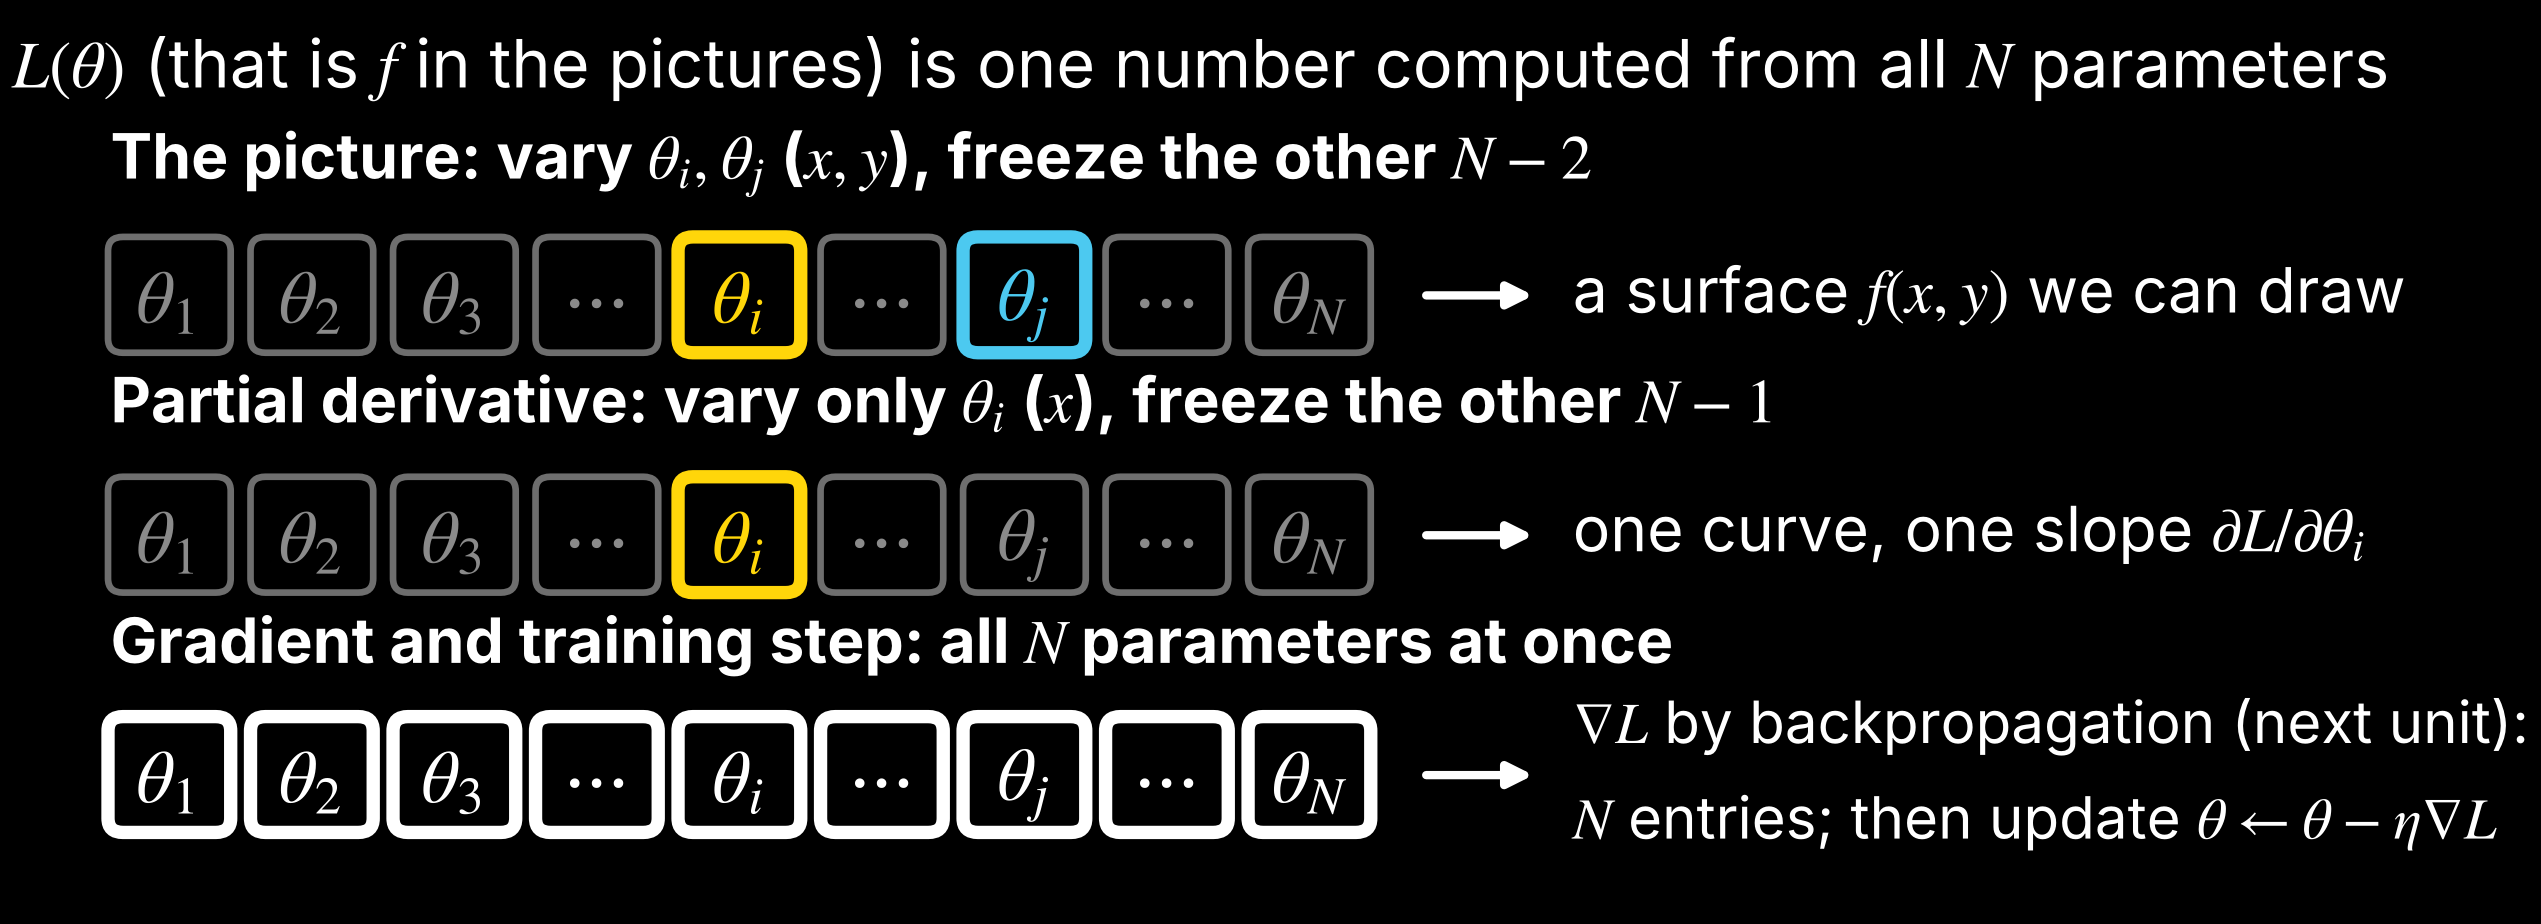
\includegraphics[width=0.97\linewidth]{figures/s1_ladder.png}}
\vfill
{\color{yellow}\rule{\linewidth}{0.5pt}}\par\vspace{1mm}
{\small\textcolor{yellow}{\textbf{Pictures vs.\ reality:}}
our pictures show two parameters at a time; every definition that follows works for all $N$.\par}
\end{frame}

\begin{frame}\FrameTitle{Slicing the loss: freeze all but one parameter}{Unit 3}
\begin{columns}[T]
\begin{column}{0.50\linewidth}
  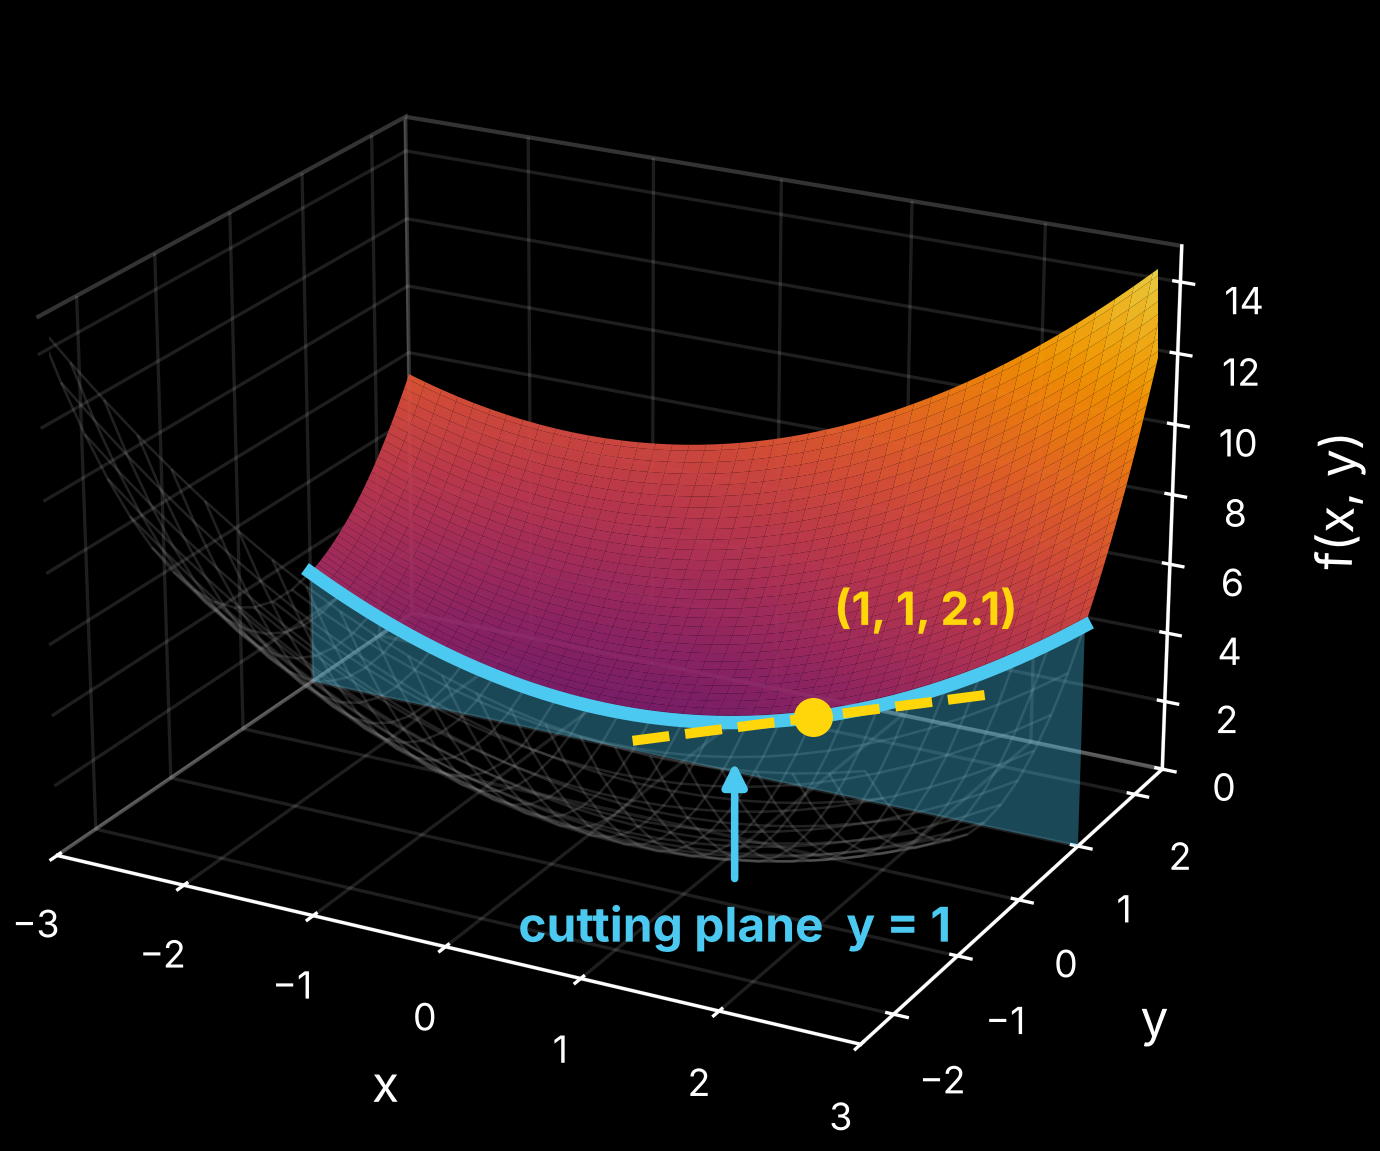
\includegraphics[width=\linewidth]{figures/s2_slice3d.png}
\end{column}
\begin{column}{0.46\linewidth}
  \begin{itemize}\small\setlength{\itemsep}{2.5mm}
    \item A surface needs two inputs, so the picture varies $x$ and $y$ and freezes the rest.
    \item Cut it with the plane $y=1$: only $x$ varies, and what is left is an ordinary curve.
    \item Its slope at the yellow point is the partial derivative $\partial f/\partial x$.
  \end{itemize}
\end{column}
\end{columns}
\vfill
{\color{yellow}\rule{\linewidth}{0.5pt}}\par\vspace{1mm}
{\small\textcolor{yellow}{\textbf{In an LLM:}} pick one weight out of billions, freeze all the others and vary it: the loss traces a curve.\par}
\end{frame}

\begin{frame}\FrameTitle{The partial derivative}{Unit 3}
\centerline{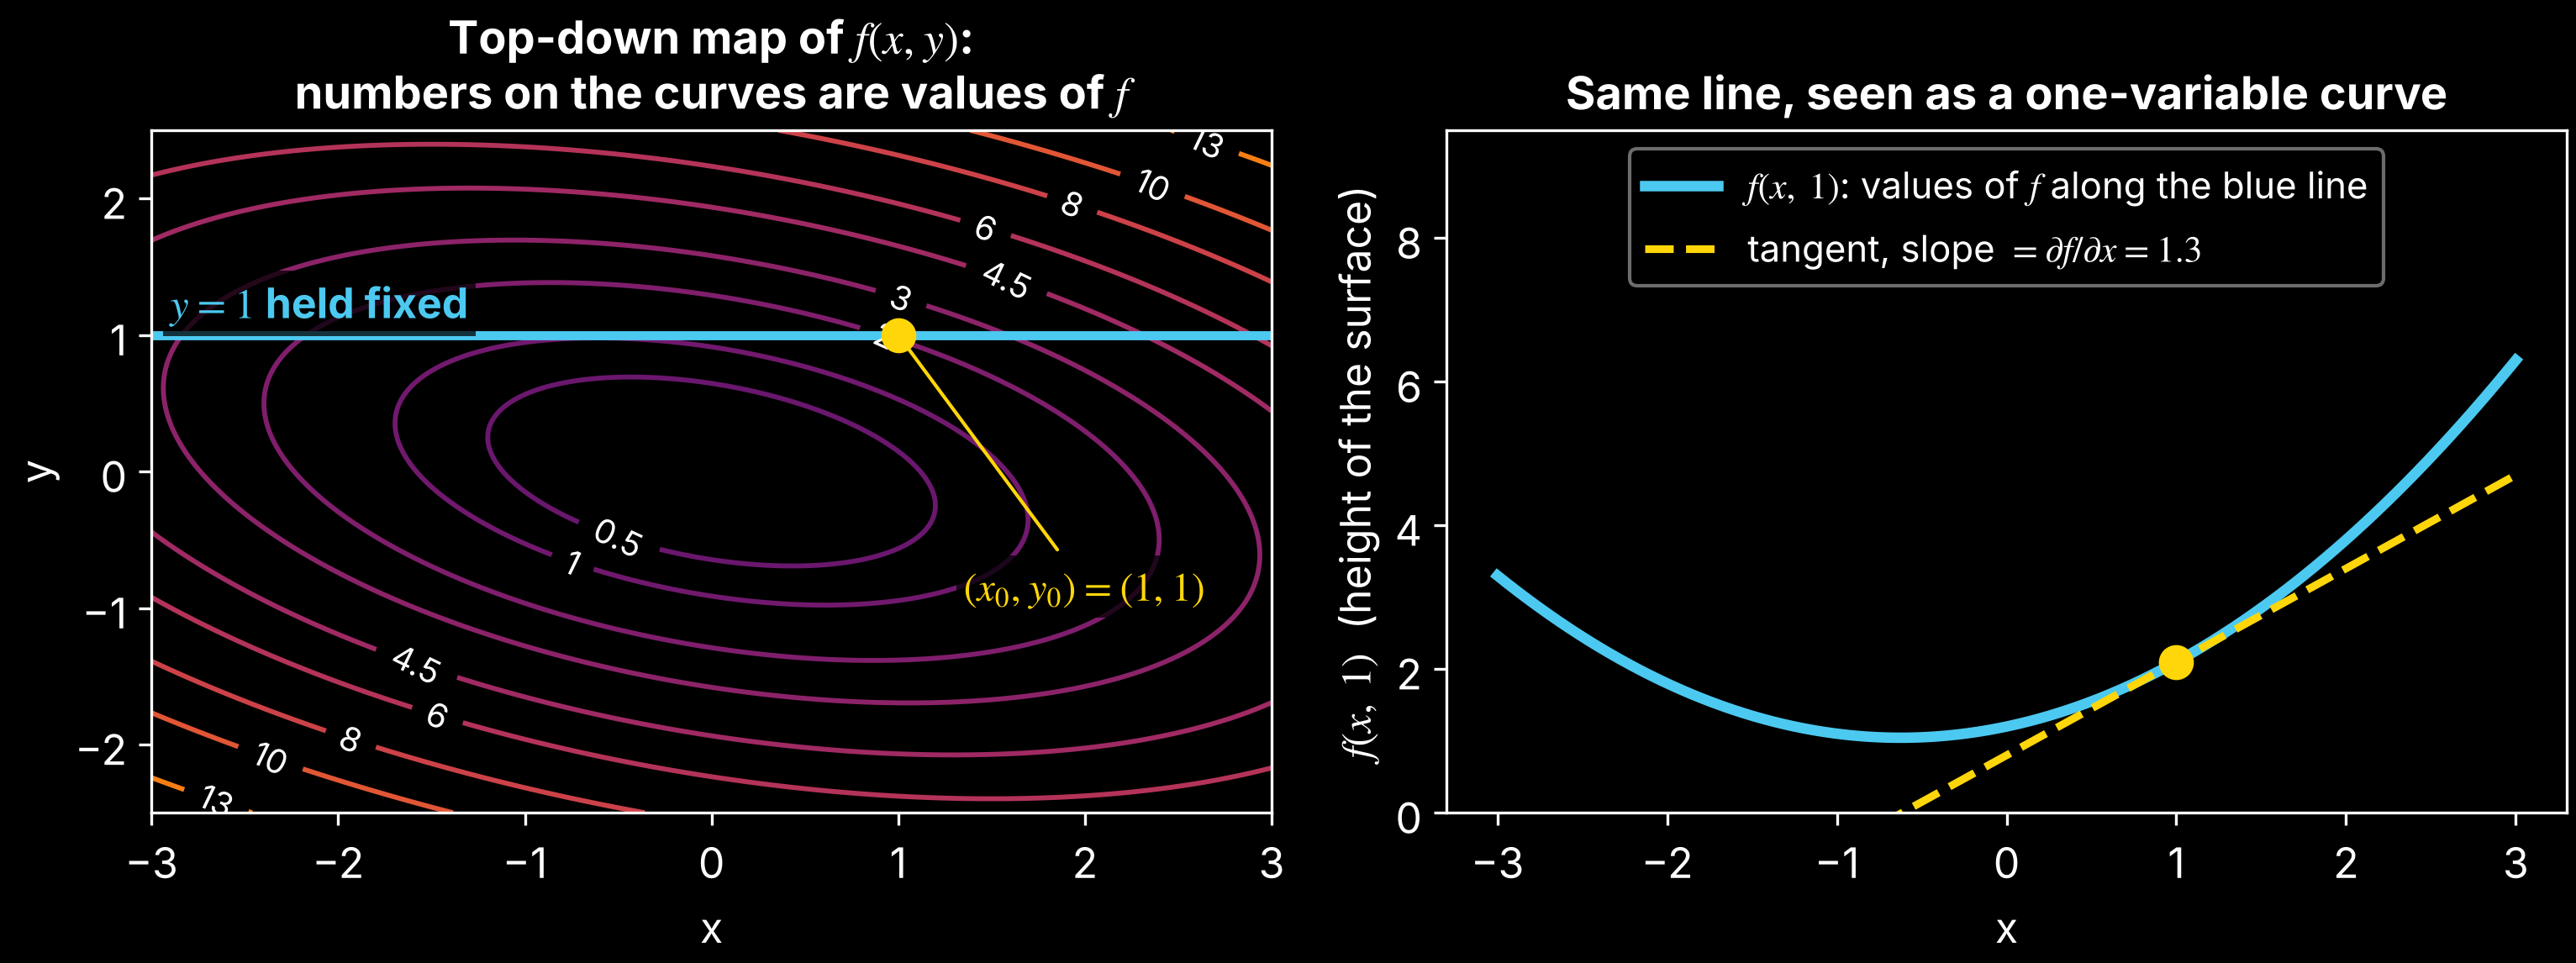
\includegraphics[width=0.90\linewidth]{figures/s3_partial.png}}
\vspace{1mm}
{\small $\displaystyle\frac{\partial f}{\partial x_j}(\symbf{x})
  =\lim_{h\to0}\frac{f(\symbf{x}+h\,\symbf{e}_j)-f(\symbf{x})}{h}$\,:
change input $j$ by a little and hold all the others fixed.\par}
\vfill
{\color{yellow}\rule{\linewidth}{0.5pt}}\par\vspace{1mm}
{\small\textcolor{yellow}{\textbf{In an LLM:}} $\partial L/\partial\theta_j$ is the sensitivity of the loss to one weight.\par}
\end{frame}

\begin{frame}\FrameTitle{The gradient}{Unit 3}
\begin{columns}[T]
\begin{column}{0.50\linewidth}
  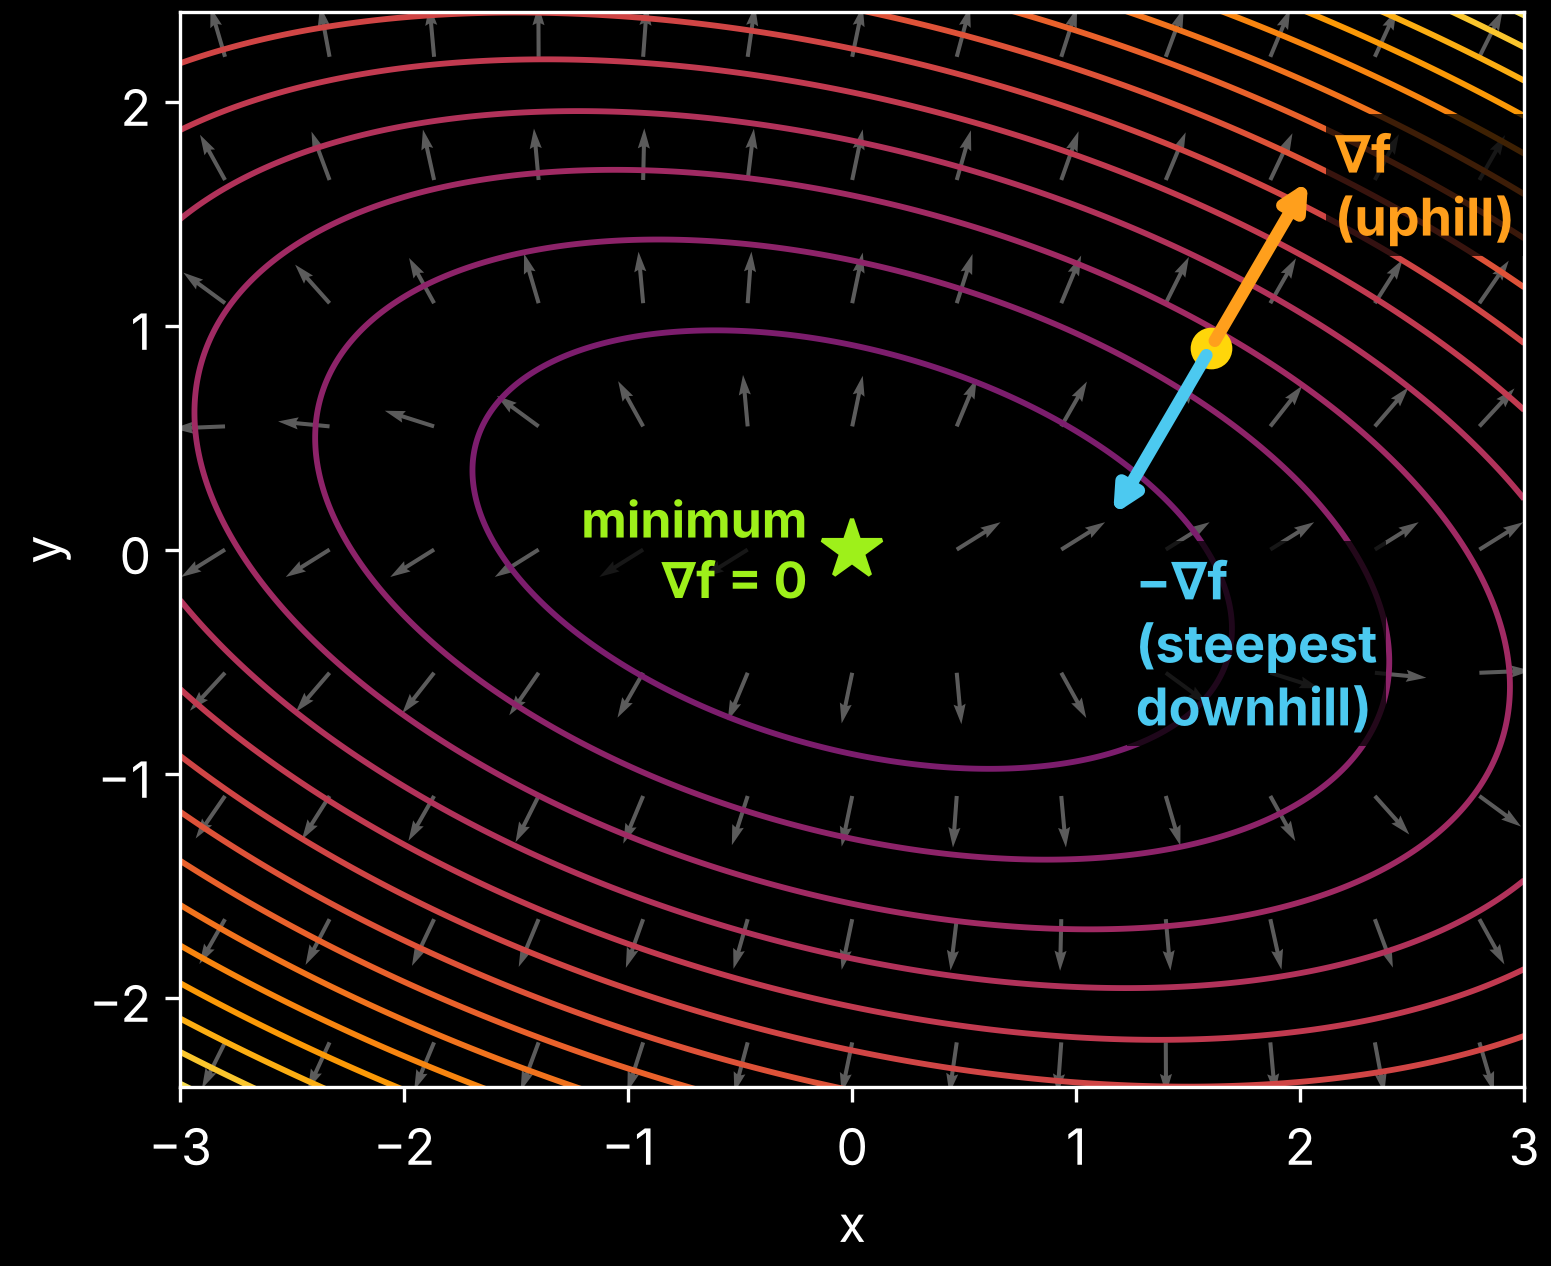
\includegraphics[width=\linewidth]{figures/s4_gradient.png}
\end{column}
\begin{column}{0.47\linewidth}
  \begin{itemize}\small\setlength{\itemsep}{2.5mm}
    \item Collect the partials into one vector with the same shape as the input:
      $\nabla f(\symbf{x})=\bigl[\partial f/\partial x_1,\dots,\partial f/\partial x_n\bigr]^{\intercal}$.
    \item $\nabla f$ points in the direction of fastest increase and is perpendicular to the contour lines.
    \item So $-\nabla f$ is the steepest way downhill.
  \end{itemize}
\end{column}
\end{columns}
\vfill
{\color{yellow}\rule{\linewidth}{0.5pt}}\par\vspace{1mm}
{\small\textcolor{yellow}{\textbf{In an LLM:}} $\nabla L$ has one entry per parameter, billions in all; $-\nabla L$ is the direction of steepest decrease.\par}
\end{frame}

\begin{frame}\FrameTitle{Local linearity and the downhill step}{Unit 3}
\centerline{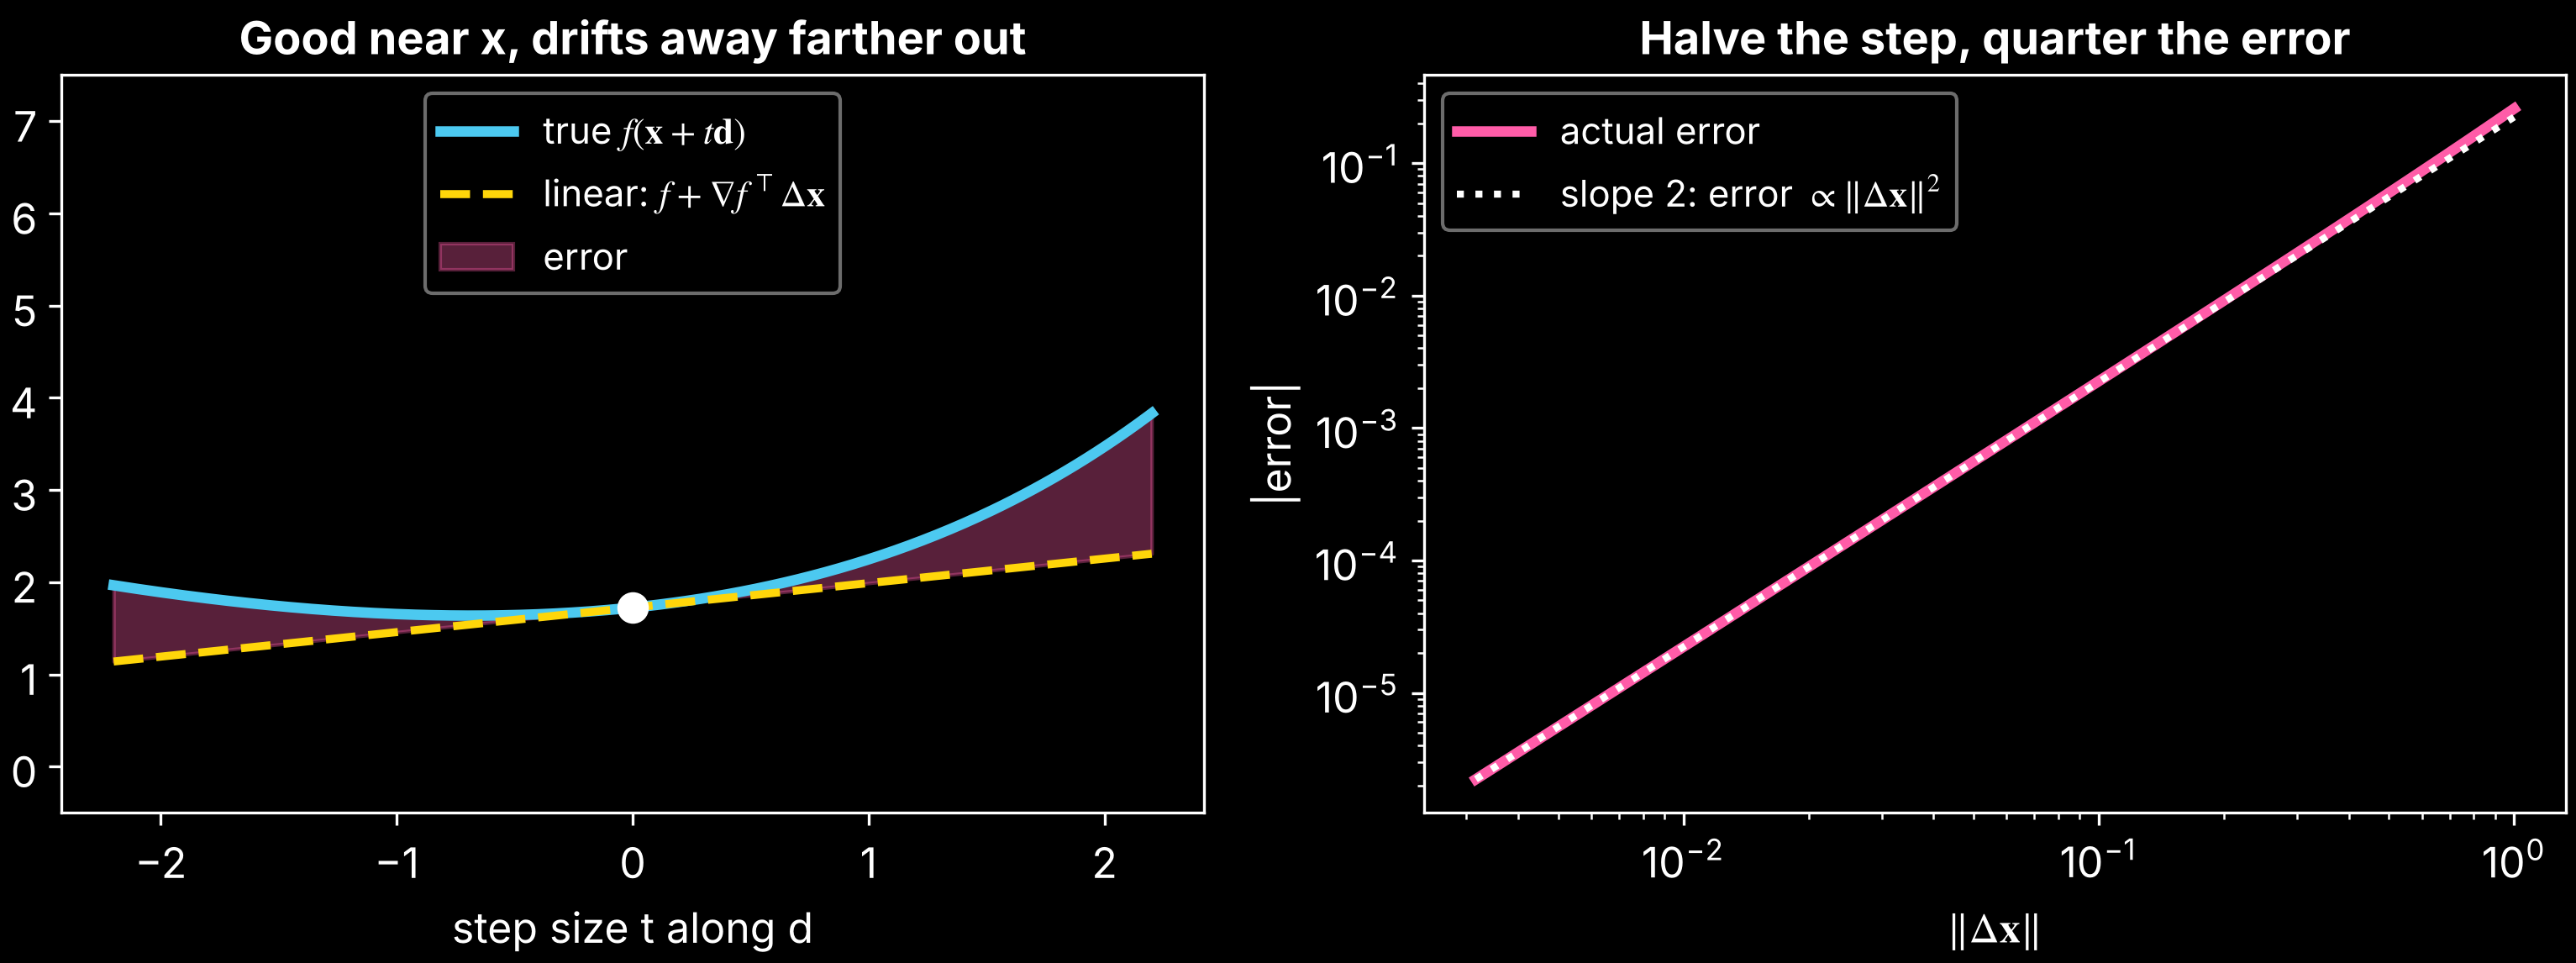
\includegraphics[width=0.90\linewidth]{figures/s5_linearity.png}}
\vspace{1mm}
{\small $f(\symbf{x}+\Delta\symbf{x})\approx f(\symbf{x})+\nabla f(\symbf{x})^{\intercal}\Delta\symbf{x}$.
Take $\Delta\symbf{x}=-\eta\,\nabla f$: then $\Delta f\approx-\eta\,\lVert\nabla f\rVert^{2}$,
a decrease for small $\eta$.\par}
\vfill
{\color{yellow}\rule{\linewidth}{0.5pt}}\par\vspace{1mm}
{\small\textcolor{yellow}{\textbf{In an LLM:}} $\symbf{\theta}\leftarrow\symbf{\theta}-\eta\nabla L$ lowers $L$ when the step is small enough; in practice $\nabla L$ is estimated on a batch of text.\par}
\end{frame}

\begin{frame}\FrameTitle{A zero gradient does not certify a minimum}{Unit 3}
\centerline{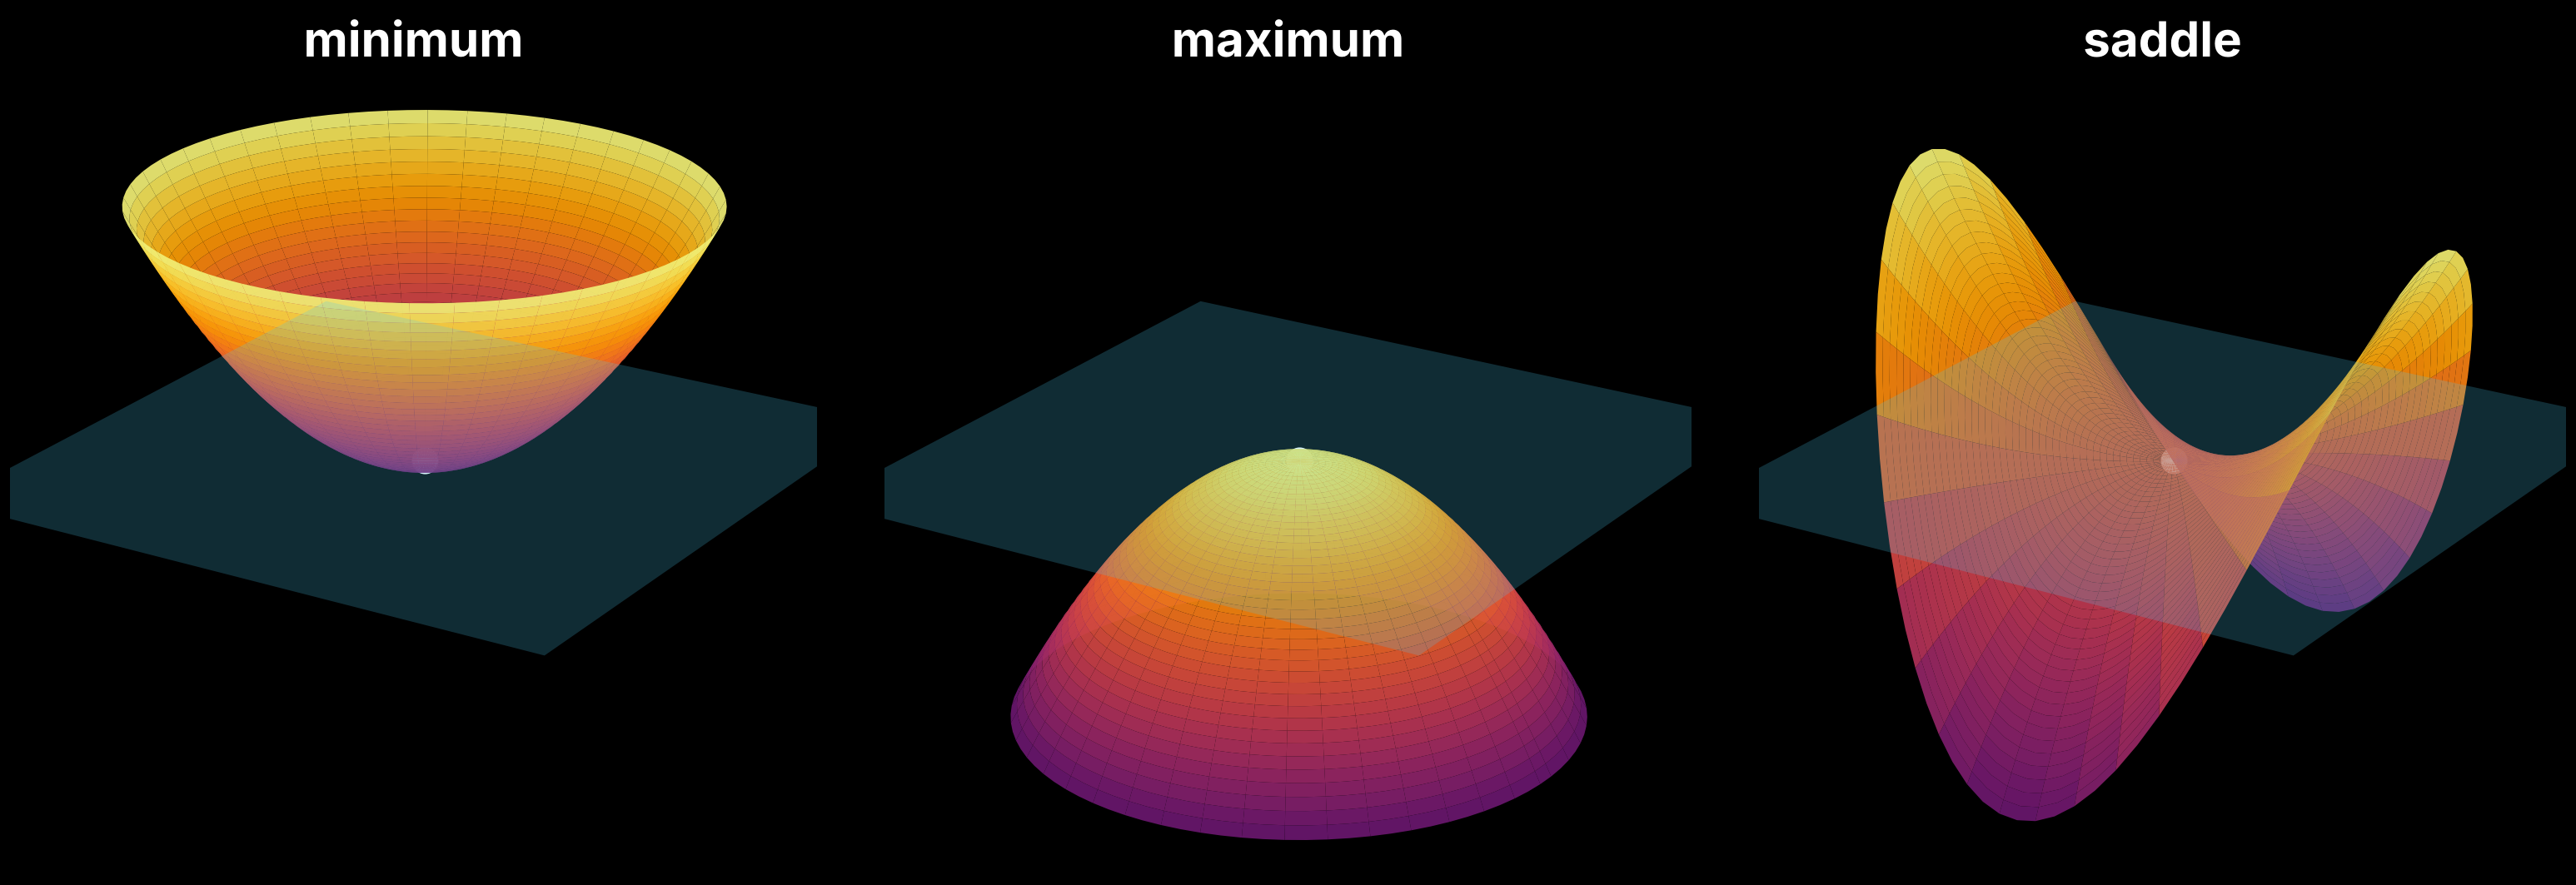
\includegraphics[width=0.96\linewidth]{figures/s7_critical.png}}
\vspace{1mm}
{\small At any minimum, maximum or saddle, $\nabla f=\symbf{0}$; the Hessian (coming later)
tells them apart. The cyan plane is the flat tangent plane at the critical point.\par}
\vfill
{\color{yellow}\rule{\linewidth}{0.5pt}}\par\vspace{1mm}
{\small\textcolor{yellow}{\textbf{In an LLM:}} training stops when the compute budget runs out, not at an exact minimum; in high dimensions, saddles are plausibly far more common than local minima.\par}
\end{frame}

%% ---------------------------------------------------------------
%% Gradients in Multiple Dimensions
\begin{frame}\FrameTitle{Gradients in Multiple Dimensions}{Unit 3}
    \begin{itemize}
        \item \textbf{Partial derivative.} $\partial f/\partial x_j$: change one
              input, hold all the others fixed.
        \item \textbf{Gradient.} Collect the partials into a vector with the
              same shape as the input:
              $\nabla f(\symbf{x}) = \bigl[\partial f/\partial x_1, \dots,
              \partial f/\partial x_n\bigr]^\top$.
        \item \textbf{Local linearity.}
              $f(\symbf{x}+\Delta\symbf{x}) \approx f(\symbf{x})
              + \nabla f(\symbf{x})^\top \Delta\symbf{x}$.
        \item \textbf{Steepest ascent.} $\nabla f$ points in the direction of
              fastest increase and is perpendicular to the contour lines, so
              $-\nabla f$ is the steepest way downhill. At a minimum,
              $\nabla f = \symbf{0}$.
        \item \textbf{Jacobian.} For $\symbf{f}:\mathbb{R}^n \to \mathbb{R}^m$,
              the $m \times n$ matrix with entries
              $J_{ij} = \partial f_i/\partial x_j$ records how every output
              responds to every input.
    \end{itemize}
\end{frame}

\begin{frame}\FrameTitle{Chain Rule in Multiple Dimensions}{Unit 3}
    \begin{itemize}
        \item \textbf{Change flows through intermediate variables.} If
              $\symbf{x} \to \symbf{y} = \symbf{g}(\symbf{x}) \to z = f(\symbf{y})$,
              a change in $x_j$ reaches $z$ through every $y_i$ that depends
              on $x_j$.
        \item \textbf{Sum over paths.}
              $\displaystyle \dfrac{\partial z}{\partial x_j}
              = \sum_i \dfrac{\partial z}{\partial y_i}\,
                       \frac{\partial y_i}{\partial x_j}$:
              multiply along each path, then add across paths.
        \item \textbf{Matrix form.} Jacobians multiply:
              $\symbf{J}_{\symbf{f}\circ\symbf{g}}(\symbf{x})
              = \symbf{J}_{\symbf{f}}\bigl(\symbf{g}(\symbf{x})\bigr)\,
                \symbf{J}_{\symbf{g}}(\symbf{x})$.
        \item \textbf{Scalar output.} When the final output is one number
              (a loss),
              $\nabla_{\symbf{x}} z = \symbf{J}_{\symbf{g}}(\symbf{x})^\top
              \nabla_{\symbf{y}} z$: the gradient is passed backward through
              the transposed Jacobian.
    \end{itemize}
\end{frame}

\begin{frame}\FrameTitle{Optimization Using Gradient Descent}{Unit 3}
    \begin{itemize}
        \item \textbf{Learning as minimization.} Training means choosing
              parameters $\symbf{\theta}$ that minimize the average loss
              $L(\symbf{\theta}) = \frac{1}{N}\sum_{n=1}^{N} \ell_n(\symbf{\theta})$.
        \item \textbf{Update rule.}
              $\symbf{\theta} \leftarrow \symbf{\theta} - \eta\,\nabla L(\symbf{\theta})$.
              By local linearity, a small step along $-\nabla L$ lowers the
              loss. If $\eta$ is too small, progress is slow; if too large,
              the steps overshoot or diverge.
        \item \textbf{Single-sample updates.}
              $\symbf{\theta} \leftarrow \symbf{\theta} - \eta\,\nabla \ell_n(\symbf{\theta})$
              for a randomly chosen example $n$. Each step is cheap, and the
              gradient is noisy but correct on average.
    \end{itemize}
\end{frame}

\begin{frame}\FrameTitle{Optimization Using Gradient Descent}{Unit 3}
    \begin{itemize}
        \item \textbf{Logistic regression.}
              $p = \sigma(\symbf{w}^\top\symbf{x} + b)$ with cross-entropy loss
              gives $\nabla_{\symbf{w}} \ell = (p - y)\,\symbf{x}$:
              prediction error times input.
        \item \textbf{Softmax regression.}
              $\symbf{p} = \operatorname{softmax}(\symbf{W}\symbf{x} + \symbf{b})$
              with cross-entropy loss gives
              $\nabla_{\symbf{W}} \ell = (\symbf{p} - \symbf{y})\,\symbf{x}^\top$
              for one-hot $\symbf{y}$, the same pattern extended to $K$ classes.
              Both losses are convex, so every local minimum is a global one.
    \end{itemize}
\end{frame}

\begin{frame}\FrameTitle{Backpropagation}{Unit 3}
    \begin{itemize}
        \item \textbf{Computational graph.} The model and loss are written as a
              chain of simple operations. Each node needs only its own local
              derivative.
        \item \textbf{Forward, then backward.} The forward pass computes and
              stores every intermediate value. The backward pass applies the
              chain rule from the loss toward the inputs, reusing those stored
              values.
        \item \textbf{Error signals.} Each node receives
              $\partial L/\partial(\text{node})$ from the nodes it feeds.
              When a value feeds several nodes, the incoming signals add.
        \item \textbf{Efficiency.} One backward pass gives the gradient for
              every parameter, at a cost comparable to one forward pass.
    \end{itemize}
\end{frame}

\begin{frame}\FrameTitle{Backpropagation}{Unit 3}
    \begin{itemize}
        \item \textbf{Multi-layer perceptron.} With
            $\symbf{z}_1 = \symbf{W}_1\symbf{x} + \symbf{b}_1$,
            $\symbf{h} = \phi(\symbf{z}_1)$,
            $\symbf{p} = \operatorname{softmax}(\symbf{W}_2\symbf{h} + \symbf{b}_2)$:
                $$\symbf{\delta}_2 = \symbf{p} - \symbf{y},$$
                $$\nabla_{\symbf{W}_2} L = \symbf{\delta}_2 \symbf{h}^\top,$$
                $$\symbf{\delta}_1 = (\symbf{W}_2^\top \symbf{\delta}_2) \odot \phi'(\symbf{z}_1),$$
                $$\nabla_{\symbf{W}_1} L = \symbf{\delta}_1 \symbf{x}^\top$$
        \item \textbf{Non-convexity.} Hidden layers make the loss non-convex.
              Gradient descent reaches a local solution, and that solution
              depends on the initialization.
    \end{itemize}
\end{frame}

\begin{frame}\FrameTitle{Reference Books}{Unit 3}
    \begin{itemize}
        \item Michael Nielsen, \emph{Neural Networks and Deep Learning}\\\vspace*{4pt}
            \href{http://neuralnetworksanddeeplearning.com/}{http://neuralnetworksanddeeplearning.com/}
        \vspace*{8pt}
        \item François Chollet, \emph{Deep Learning with Python},\\\vspace*{4pt}
            \href{https://www.manning.com/books/deep-learning-with-python}{https://www.manning.com/books/deep-learning-with-python}
        \item \href{https://www.3blue1brown.com/}{3Blue1Brown}\\\vspace*{4pt}
            \href{https://www.3blue1brown.com/?topic=calculus}{https://www.3blue1brown.com/?topic=calculus}
    \end{itemize}
\end{frame}

\end{document}
